%%%%%%%%%%%%%%%%%%%% book.tex %%%%%%%%%%%%%%%%%%%%%%%%%%%%%
%
% sample root file for the chapters of your "monograph"
%
% Use this file as a template for your own input.
%
%%%%%%%%%%%%%%%% Springer-Verlag %%%%%%%%%%%%%%%%%%%%%%%%%%


% RECOMMENDED %%%%%%%%%%%%%%%%%%%%%%%%%%%%%%%%%%%%%%%%%%%%%%%%%%%
\documentclass[envcountsame,envcountchap]{svmono}

% choose options for [] as required from the list
% in the Reference Guide, Sect. 2.2

\usepackage{makeidx}         % allows index generation
\usepackage{graphicx}        % standard LaTeX graphics tool
                             % when including figure files
\usepackage{multicol}        % used for the two-column index
\usepackage[bottom]{footmisc}% places footnotes at page bottom
% etc.
% see the list of further useful packages
% in the Reference Guide, Sects. 2.3, 3.1-3.3

\makeindex             % used for the subject index
                       % please use the style svind.ist with
                       % your makeindex program


%%%%%%%%%%%%%%%%%%%%%%%%%%%%%%%%%%%%%%%%%%%%%%%%%%%%%%%%%%%%%%%%%%%%%

\begin{document}

\author{\textbf{FEUP-PLOG, Turma 3MIEIC01, Grupo Hamle\_2}\\ \\
	\normalsize Faculdade de Engenharia da Universidade do Porto \\ 
	\small Rua Roberto Frias, s\/n, 4200-465 Porto, Portugal }

\title{Resolu\c{c}\~ao de Problema de Decis\~ao/Otimiza\c{c}\~ao usando
	Programa\c{c}\~ao em L\'ogica com Restri\c{c}\~oes}
\subtitle{-- Hamle --}


\maketitle



\frontmatter%%%%%%%%%%%%%%%%%%%%%%%%%%%%%%%%%%%%%%%%%%%%%%%%%%%%%%

%%%%%%%%%%%%%%%%%%%%%% pref.tex %%%%%%%%%%%%%%%%%%%%%%%%%%%%%%%%%%%%%
%
% sample preface
%
% Use this file as a template for your own input.
%
%%%%%%%%%%%%%%%%%%%%%%%% Springer-Verlag %%%%%%%%%%%%%%%%%%%%%%%%%%

\chapter*{Resumo/Abstract}

Tendo como material de estudo a programa\c{c}\~ao em l\'ogica com restri\c{c}\~oes, \'e-nos proposta a resolu\c{c}\~ao de um problema de decis\~ao relativo a um jogo de tabuleiro. Para o efeito, o nosso grupo selecionou o jogo Hamle, como objeto de trabalho.


\vspace{\fill}
\begin{flushright}\noindent
Faculdade de Engenharia da Universidade do Porto,\hfill {\it Daniel Reis}\\
Dezembro de 2015\hfill {\it Guilherme Pinto}\\
\end{flushright}
\let\cleardoublepage\clearpage
\tableofcontents

\mainmatter%%%%%%%%%%%%%%%%%%%%%%%%%%%%%%%%%%%%%%%%%%%%%%%%%%%%%%%
\chapter{Introdu\c{c}\~ao}

Neste relat\'orio estudaremos a gera\c{c}\~ao de solu\c{c}\~oes com base na programa\c{c}\~ao em l\'ogica com restri\c{c}\~oes, demonstrando os resultados obtidos e comparando os tempos de execu\c{c}\~ao para tabuleiros de diferentes dimens\~oes.\\
Relativamente ao problema abordado, o Hamle consiste num jogo de tabuleiro quadrangular (6x6), com dez pe\c{c}as pretas posicionadas em locais espec\'ificos. Por sua vez, cada uma destas pe\c{c}as apresentar\'a um n\'umero correspondente ao deslocamento que dever\'a efetuar em qualquer umas das quatro dire\c{c}\~oes poss\'iveis. Ap\'os o deslocamento, nenhuma pe\c{c}a preta poder\'a ser adjacente a outra, assim como todas as c\'elulas vazias dever\~ao estar interligadas, ou seja, nao poder\~a existir dois ou mais grupos distintos de c\'elulas vazias.\\
Quanto \`a estrutura\c{c}\~ao do relat\'orio, orientar-nos-emos por uma an\'alise detalhada \`as restri\c{c}\~oes impostas, descrevendo de seguida o c\'odigo implementado, estudando os resultados apresentados em terminal e discutindo os valores e solu\c{c}\~oes obtidas.
\chapter{Descri\c{c}\~ao do Problema}
\label{intro} % Always give a unique label
% use \chaptermark{}
% to alter or adjust the chapter heading in the running head

O problema em an\'alise deve ser abordado segundo as restri\c{c}\~oes descritas nas regras do jogo:\\
\\
\begin{itemize}
	\item Cada pe\c{c}a preta deve ser deslocada, em qualquer uma das quatro dire\c{c}\~oes poss\'iveis, o n\'umero de c\'elulas correspondente ao valor que lhe est\'a atribu\'ido.
	
	\item No final do movimento das pe\c{c}as pretas, nenhuma delas dever\'a ser adjacente a qualquer outra pe\c{c}a.
	
	\item Al\'em da restri\c{c}\~ao anterior, na conclus\~ao dos deslocamentos das pe\c{c}as, deve-se verificar que todas as c\'elulas vazias dever\~ao estar interligadas entre si, ou seja, selecionando qualquer posi\c{c}\~ao livre do tabuleiro, deve ser poss\'ivel encontrar um caminho at\'e qualquer outra c\'elula desocupada, sem saltar por cima de qualquer pe\c{c}a preta.
\end{itemize}

O alcance de uma solu\c{c}\~ao correta \'e apenas poss\'ivel recorrendo a implementa\c{c}\~ao das restri\c{c}\~oes apresentadas. Dado que qualquer uma delas \'e dependente dos resultado das restantes, \'e importante recorrer a programa\c{c}\~ao l\'ogica com restr\c{c}\~oes de modo a determinar uma resolu\c{c}\~ao r\'apida e eficaz.
\chapter{Abordagem}

Neste cap\'itulo ser\'a realizada uma minuciosa an\'alise ao jogo Hamle e ao m\'etodo de resolu\c{c}\~ao implementado. \\
Come\c{c}aremos por descrever as vari\'aveis de decis\~ao e seus respetivos dom\'inios, seguidas de uma avalia\c{c}\~ao das restri\c{c}\~oes a serem trabalhadas. Ser\'a ainda indicada a forma de avalia\c{c}\~ao da solu\c{c}\~ao obtida bem como a estrat\'egia de pesquisa aplicada ao $labeling$, no c\'alculo das poss\'iveis solu\c{c}\~oes.

\section{Vari\'aveis de Decis\~ao}

Como variavel de decis\~ao, \'e gerada, na fun\c{c}\~ao $solution$, uma lista denominada $Result$ a qual ter\'a a dimens\~ao de um tabuleiro, simulando a jun\c{c}\~ao de uma linha do tabuleiro ao final da anterior, isto \'e, tendo como exemplo um tabuleiro NxN, temos que $length(Result, Length)$, onde $Length = N*N$.\\
O dom\'inio da vari\'avel $Result$ ser\'a compreendido entre 0 e $N-1$, sendo que 0 representar\'a as c\'elulas vazias e os algarismos compreendidos entre 1 e $N-1$ corresponder\~ao \`a desloca\c{c}\~ao respetiva a cada pe\c{c}a preta presente no tabuleiro original. Sendo assim, a cada algarismo $V$ presente num dado \'indice $I$ da lista $Result$, ent\~ao, necess\'ariamente, existir\'a na lista original (representativa do estado inicial do tabuleiro), o mesmo valor $N$ no \'indice $I + N*V$ (deslocamento para baixo), no \'indice $I - N*V$ (deslocamento para cima), no \'indice $I + V$ (deslocamento para a direita) ou no \'indice $I - V$ (deslocamento para a esquerda). N\~ao pode deixar de ser referido que no deslocamento horizontal, o \'indice de destino dever\'a corresponder \`a mesma linha do \'indice de origem, pelo que $floor(I\small{destino} / N) = floor(I\small{origem} / N)$.\\ \\ \\ \\ \\ \\ \\ 

\section{Restri\c{c}\~oes}

No presente subcap\'itulo, descreveremos a implementa\c{c}\~ao das diversas restri\c{c}\~oes que constituem o problema da determina\c{c}\~ao de solu\c{c}\~oes para o jogo Hamle. Para qualquer umas das restri\c{c}\~oes foi criada uma fun\c{c}\~ao auxiliar para o respetivo c\'alculo ou verifica\c{c}\~ao.

\subsection{Pe\c{c}as n\~ao-adjacentes}
Esta \'e a restri\c{c}\~ao mais simples das que consistem o jogo. 
\\ \\
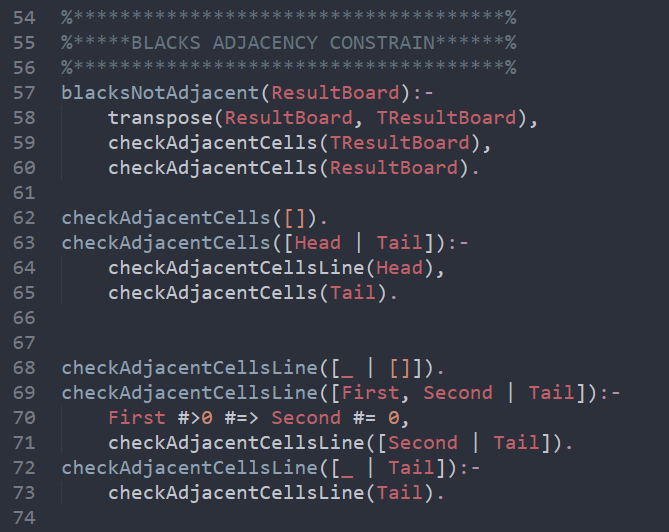
\includegraphics[scale=0.5]{no-adjacents.png}
\\ \\
Tendo como argumento $ResultBoard$ (uma lista de listas respetiva \`a divis\~ao da lista de vari\'aveis $Result$, sendo que cada sublista representa uma linha do tabuleiro), temos como objetivo garantir que nenhuma posi\c{c}\~ao com valor superior a 0 tenha na sua proximidade outro valor igualmente superior a 0. Desse modo, ao percorrer uma linha do tabuleiro (sublista de $ResultBoard$), impomos que, dada uma posi\c{c}\~ao, referente a uma pe\c{c}a preta, dever\'a ser seguida de um espa\c{c}o em branco (valor 0). Uma vez que esta condi\c{c}\~ao se verifica tanto na horizontal como na vertical, gera-se uma matriz transposta a $ResultBoard$ que posteriormente ser\'a verificada com as restri\c{c}\~ao em an\'alise.
\\ \\ \\ \\ \\ \\ \\ \\

\subsection{Movimento de pe\c{c}as pretas}
Relativamente ao movimento das pe\c{c}as pretas, podemos dividir a restri\c{c}\~ao em duas fases: a verifica\c{c}\~ao das possibilidades de desloca\c{c}\~ao de cada pe\c{c}a e a respetiva valida\c{c}\~ao e coloca\c{c}\~ao em tabuleiro.
\\ \\
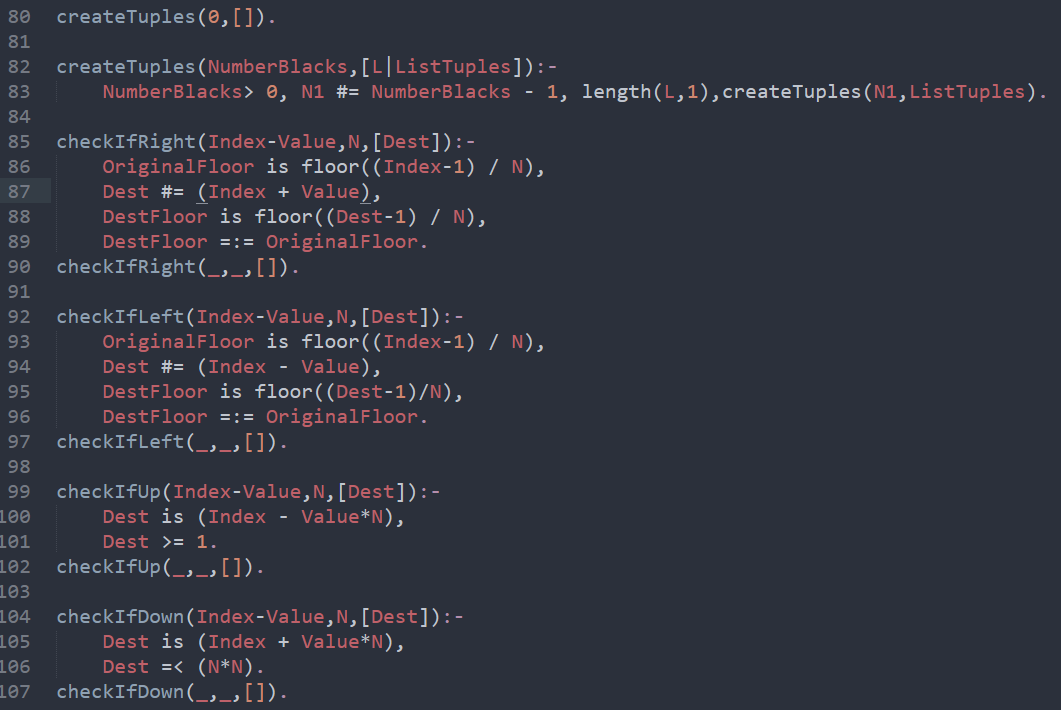
\includegraphics[scale=0.5]{movement-checkers.png}
\\ 
Nestas fun\c{c}\~oes s\~ao recriadas as possiveis posi\c{c}\~oes que cada pe\c{c}a poder\'a ocupar, dependendo da c\'elula onde se encontra e da dire\c{c}\~ao na qual se poder\'a deslocar. Estas posi\c{c}\~oes a serem determinadas s\~ao calculadas com base no \'indice de cada c\'elula, pelo que se recorre \`a fun\c{c}\~ao $floor/1$ para considerar que, em caso de deslocamento horizontal, o indice de origem corresponde \`a mesma linha de tabuleiro que o \'indice de destino.
\\ \\
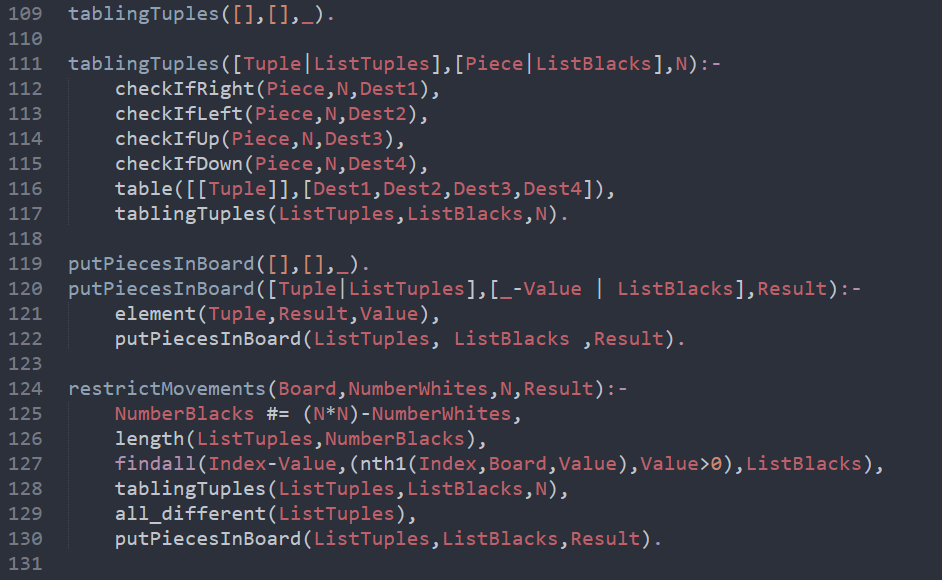
\includegraphics[scale=0.4]{movement-validators.png}
\\ \\
Ap\'os a determina\c{c}\~ao dos poss\'iveis destinos para cada pe\c{c}a preta, procede-se \`a coloca\c{c}\~ao de cada uma no seu novo local recorrendo ao $table$, que nos permite criar um subdom\'inio relativo a cada objeto, com as diferentes posi\c{c}\~oes para onde se poder\'a mover. Neste momento, \'e tamb\'em restringida a possibilidade de quaisquer pe\c{c}as ocuparem a mesma c\'elula.

\subsection{Interconectividade das c\'elulas vazias}
Embora o conceito de interconectividade n\~ao seja complicado de assimilar, n\~ao fomos capazes de implementar corretamente a restri\c{c}\~ao pretendida neste ponto.
Na imagem seguinte apresentamos o algoritmo que nos permite detetar o n\'umero de c\'elulas vazias \`as quais podemos aceder, partindo de uma posi\c{c}\~ao livre.
\\ \\ 
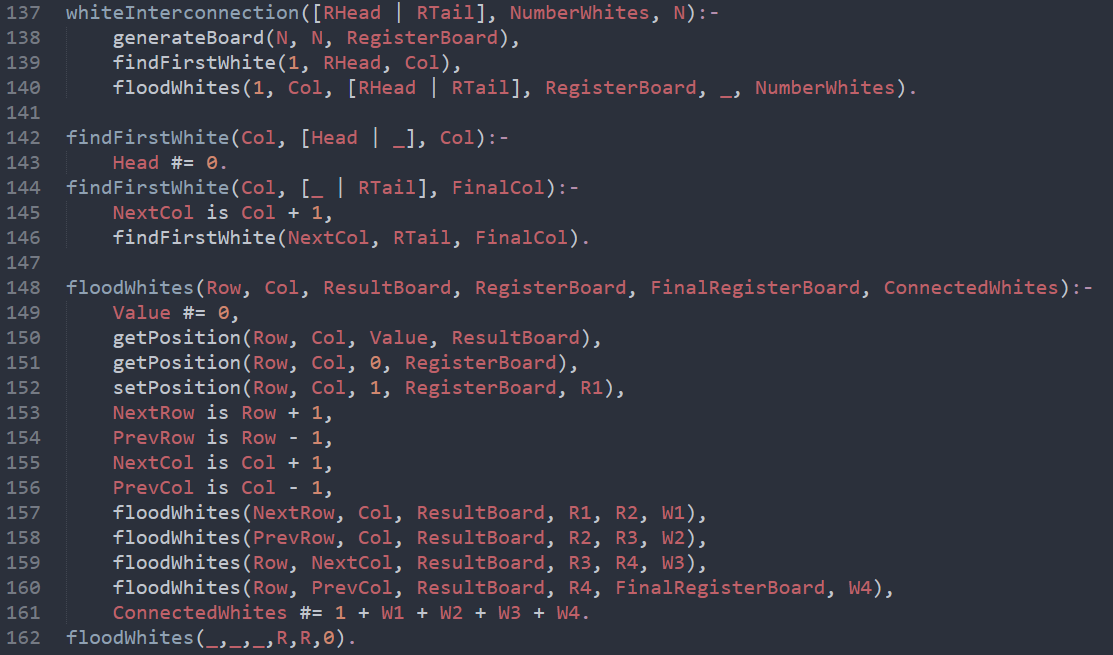
\includegraphics[scale= 0.5]{white-interconnection.png}
\\ \\ \\ \\ \\
O objetivo do nosso grupo seria, ap\'os detetar a primeira c\'elula vazia da primeira linha de tabuleiro, expandir a procura atrav\'es das c\'elulas desocupadas na vizinhan\c{c}a dessa primeira posi\c{c}\~ao, recorrendo ao aux\'ilio de um tabuleiro de registo, que nos identificaria as c\'elulas anteriormente visitadas durante o processo.\\
Tendo testado o algoritmo, podemos assegurar que se encontra funcional, embora n\~ao seja vi\'avel ao pretendido neste projeto.

\section{Fun\c{c}\~ao de Avalia\c{c}\~ao}
Ap\'os a execu\c{c}\~ao das restri\c{c}\~oes e alcance de uma solu\c{c}\~ao que as satisfa\c{c}a, ser\'a poss\'ivel visualizar um novo tabuleiro com a respetiva movimenta\c{c}\~ao de cada pe\c{c}a preta. Tal poder\'a ser observado uma vez que cada pe\c{c}a conservar\'a o seu valor de deslocamento, assim como no tabuleiro original.

\section{Estrat\'egia de Pesquisa}
Foi utilizada, como estrat\'egia de etiquetagem, o modo $default$ da fun\c{c}\~ao $labeling$, ou seja, recorre-se \`as op\c{c}\~oes $leftmost$, $step$, $up$ e $all$.


%%%%%%%%%%%%%%%%%%%%%% chapter.tex %%%%%%%%%%%%%%%%%%%%%%%%%%%%%%%%%
%
% sample chapter
%
% Use this file as a template for your own input.
%
%%%%%%%%%%%%%%%%%%%%%%%% Springer-Verlag %%%%%%%%%%%%%%%%%%%%%%%%%%

\chapter{Chapter Heading}
\label{intro} % Always give a unique label
% use \chaptermark{}
% to alter or adjust the chapter heading in the running head

Your text goes here. Separate text sections with the standard \LaTeX\
sectioning commands.

\section{Section Heading}
\label{sec:1}
% Always give a unique label
% and use \ref{<label>} for cross-references
% and \cite{<label>} for bibliographic references
% use \sectionmark{}
% to alter or adjust the section heading in the running head
Your text goes here. Use the \LaTeX\ automatism for your citations
\cite{monograph}.

\subsection{Subsection Heading}
\label{sec:2}
Your text goes here.

\begin{equation}
\vec{a}\times\vec{b}=\vec{c}
\end{equation}

\subsubsection{Subsubsection Heading}
Your text goes here. Use the \LaTeX\ automatism for cross-references as
well as for your citations, see Sect.~\ref{sec:1}.

\paragraph{Paragraph Heading} %
Your text goes here.

\subparagraph{Subparagraph Heading.} Your text goes here.%
%
\index{paragraph}
% Use the \index{} command to code your index words
%
% For tables use
%
\begin{table}
\centering
\caption{Please write your table caption here}
\label{tab:1}       % Give a unique label
%
% For LaTeX tables use
%
\begin{tabular}{lll}
\hline\noalign{\smallskip}
first & second & third  \\
\noalign{\smallskip}\hline\noalign{\smallskip}
number & number & number \\
number & number & number \\
\noalign{\smallskip}\hline
\end{tabular}
\end{table}
%
%
% For figures use
%
\begin{figure}
\centering
% Use the relevant command for your figure-insertion program
% to insert the figure file.
% For example, with the option graphics use
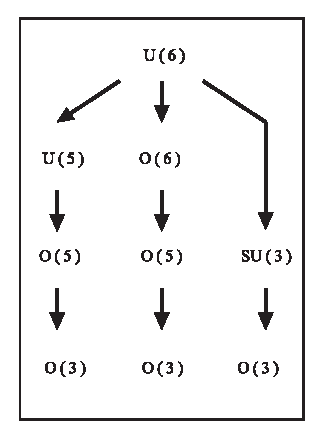
\includegraphics[height=4cm]{figure.eps}
%
% If not, use
%\picplace{5cm}{2cm} % Give the correct figure height and width in cm
%
\caption{Please write your figure caption here}
\label{fig:1}       % Give a unique label
\end{figure}
%
% For built-in environments use
%
\begin{theorem}
Theorem text goes here.
\end{theorem}
%
% or
%
\begin{lemma}
Lemma text goes here.
\end{lemma}
%
%
% Problems or Exercises should be sorted chapterwise
\section*{Problems}
\addcontentsline{toc}{section}{Problems}
%
% Use the following environment.
% Don't forget to label each problem;
% the label is needed for the solutions' environment
\begin{prob}
\label{prob1}
The problem\footnote{Footnote} is described here. The
problem is described here. The problem is described here.
\end{prob}

\begin{prob}
\label{prob2}
\textbf{Problem Heading}\\
(a) The first part of the problem is described here.\\
(b) The second part of the problem is described here.
\end{prob}



%

%\appendix
%\include{appendix}

\backmatter%%%%%%%%%%%%%%%%%%%%%%%%%%%%%%%%%%%%%%%%%%%%%%%%%%%%%%%
%
\chapter*{Solutions}
\addcontentsline{toc}{chapter}{Solutions}
\markboth{Solutions}{Solutions}

\section*{Problems of Chapter~\ref{intro}}

\begin{sol}{prob1}
The solution is revealed here.
\end{sol}


\begin{sol}{prob2}
\textbf{Problem Heading}\\
(a) The solution of first part is revealed here.\\
(b) The solution of second part is revealed here.
\end{sol}


%%%%%%%%%%%%%%%%%%%%%%%% referenc.tex %%%%%%%%%%%%%%%%%%%%%%%%%%%%%%
% sample references
% "computer science"
%
% Use this file as a template for your own input.
%
%%%%%%%%%%%%%%%%%%%%%%%% Springer-Verlag %%%%%%%%%%%%%%%%%%%%%%%%%%

%
% BibTeX users please use
% \bibliographystyle{}
% \bibliography{}
%
% Non-BibTeX users please use
\begin{thebibliography}{99.}
%
% and use \bibitem to create references.
%
% Use the following syntax and markup for your references
%
% Monographs
\bibitem{monograph} Kajan E (2002)
Information technology encyclopedia and acronyms. Springer, Berlin
Heidelberg New York

% Contributed Works
\bibitem{contribution} Broy M (2002) Software engineering -- From
auxiliary to key technologies. In: Broy M, Denert E (eds)
Software Pioneers. Springer, Berlin Heidelberg New York

% Journal
\bibitem{journal} Che M, Grellmann W, Seidler S (1997)
Appl Polym Sci 64:1079--1090

% Theses
\bibitem{thesis} Ross DW (1977) Lysosomes and storage diseases. MA
Thesis, Columbia University, New York

\end{thebibliography}

\printindex

%%%%%%%%%%%%%%%%%%%%%%%%%%%%%%%%%%%%%%%%%%%%%%%%%%%%%%%%%%%%%%%%%%%%%%

\end{document}





